\clearpage
\begin{flushright}
	\textit{Лекция №14}
	\textit{2015.11.03}
\end{flushright}

\paragraph{Задача читатели – писатели}. Бытовая интерпретация – система продажи билетов на самолеты, когда бронируются места, конкретный день и рейс. Состоит из 2 этапов:
\begin{enumerate}
    \item чтение информации, указываем вылет прилет, дату …
    \item бронирование.
\end{enumerate} 

Место – критическая переменная. Когда бронируем –  мы выступаем как писатель.   
Писатель (по конкретной разделяемой переменной) может быть только один.

\subsection{Монитор Хоара}
Если кто то пишет или есть писатели, ждущие своей очереди, то читатель переводится в состояние ожидание на переменной типа условие \verb|canread|.  Если читатель минует блокировку, то увеличивается активных читателей и читатель посылает сигнал читателям, которые ожидают своей очереди на чтение. Цепная реакция читателей. Каждый читатель инициирует других читателей. Читатели могу работать параллельно. По завершении чтения процесс вызывает \verb|stopread()|, уменьшается кол-во активных читателей, и если их число равно 0, то посылается сигнал – можно писать. Проверка очереди гарантирует, что не будет бесконечного откладывания ???. 
Когда процесс писатель начинается, вызывается \verb|startwrite()|.
Бесконечное откладывание читателей исключается в \verb|stopwrite()|. 
Эти функции есть в UNIX. 
Если писатель готов писать – надо дать ему эту возможность.

\begin{figure}[H]
    \centering
    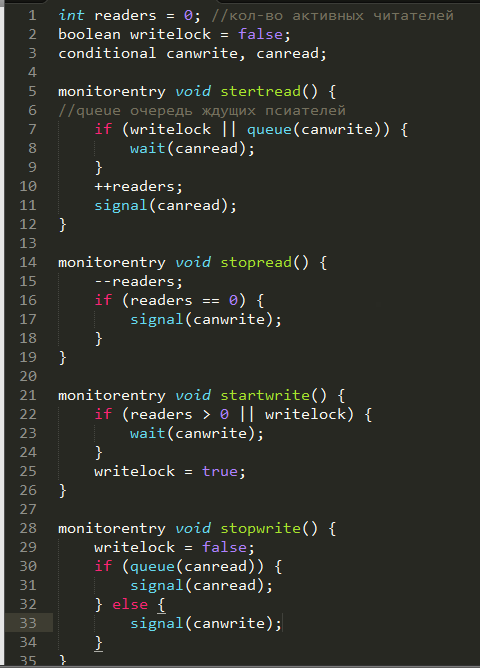
\includegraphics[width=\textwidth]{listing/1.png}
    \caption{listing}
\end{figure}

\paragraph{ЛР №3}  максимально использовать основное свойство набора семафоров – одной неделимой операцией можно изменять все или часть семафоров набора.  Объявляем набор из трех семафоров. Наборы семафоров семантически реализованы как массивы. Два семафора – как считающие, и один – как бинарный.\\ 
1) Реализация производство-потребление на трех семафорах решение Дейкстры.\\
2) Читатели-писатели на семафорах и разделяемой памяти.\\
Монитор Хоара читатели – писатели под Windows под win32 без оконного интерфейса. Открываем книгу \cite{Rih_Win_prof}. Можно посмотреть про потоки. Реализуем на event. В Windows – с автосбросом и со сбросом вручную. Потребуются оба типа. Нужно подумать, как использовать мьютекс.\\ 
Моделируем простейшую ситуацию, когда потоки разделяют одну глобальную переменную. Каждый писатель просто инкрементирует разделяемую переменную. При работе программы должно быть видно: какой писатель,  что записал и что читают читатели. Чтобы они не работали последовательно, ставим рандомные задержки.


\section{Проблема спящего парикмахера}

(с точки зрения асинхронных процессов и ресурсов, которые эти процессы захватывают). Относится к классическим задачам в синхронизации. Аналогия – над гипотетическим одним парикмахером. Одно рабочее место и приемная с несколькими стульями. Когда парикмахер заканчивает подстригать клиента и идет в приемную, чтобы посмотреть, если ли ждущие клиенты. Если есть – то приглашает одного и начинает стричь. Если ждущих клиентов нет – то возвращается в свое кресло и спит. Каждый приходящий клиент смотрит, что делает парикмахер. Если спит – то будет его и садится в кресло, если парикмахер работает – то клиент идет в приемную, и если в ней есть свободный стул и занимает её. Если стула нет – клиент уходит. Нет критических ситуация при беглом рассмотрении, но если рассмотреть подробнее, то можно выделить критические действия, связанные с тем, что действия клиентов и парикмахера занимают неизвестное кол-во времени и они - параллельные. Например: клиент входит и видит, что парикмахер работает, тогда он идет в приемную. Пока он идет со своей скоростью, а парикмахер заканчивает и идет в приемную быстрее чем клиент, придя – обнаруживают пустую приемную, идет спать, а клиент уверенный что парикмахер работает, идет ждать. Другой пример: два клиента могут прийти в одной и тоже время, когда в приемной есть один свободный стул. Они видят, что парикмахер работают и оба пытаются занять единственный стул. 

Рандеву – особый тип взаимодействия. В классическом виде реализована в языке Ада. (применяется в банковском деле и в аэропортах). Работа с параллельными процессами в языке Ада ?? называется task. Task – специальный вид модуля, который может работать независимо от других модулей. Task имеют средство связи друг с другом. Task имеют спецификацию и тело. Задачи не могут быть оттранслированы самостоятельно, они связываются между собой при помощи входов entry. Если одна задача выдала обращение к входу и оно принимается другой задачей, то обе задачи теряют свою независимость, т.е. между ними устанавливается рандеву. Пока рандеву действует – они синхронизированы. В механизме рандеву отсутствует симметрия. Если одна задача инициирует рандеву, то вторая задача может принять, а может и не принять вызов первой задачи. Рандеву происходит только тогда, когда задача, к которой произошел вызов – принимает вызов. Рандеву начинается с согласования фактических и формальных параметров. Далее оно продолжается выполнением операторов, которые располагаются между ключевыми словами do – be end. Во время рандеву task’и могут обмениваться информацией через список параметров. Последовательность операторов выполняется от имени обоих задач. В результате синхронизированные задачи получают результат выполнения последовательности операторов одновременно!!!!

\paragraph{Итог:} рассмотрели блокирующие и освобождающие системные вызовы, в отличие от рандеву Ады, всё что мы рассмотрели – блокирующие и ???. При этом в системах самым общим способом взаимодействия является передача сообщений. Система также предоставляет системные вызовы для передачи сообщений (send receive). Передача сообщений в самом общем виде.

\paragraph{Проблемы при передаче сообщений}: рассмотрим два процесса, выполняющихся параллельно.  Возьмем один процесс на одном компе, другой на другом. Они должны обменяться сообщениями. Один процесс выполнялся некоторое время. В какой то момент времени он посылает сообщение-запрос другому процессу, который также выполняется и что то делает. 

\begin{figure}[H]
    \centering
    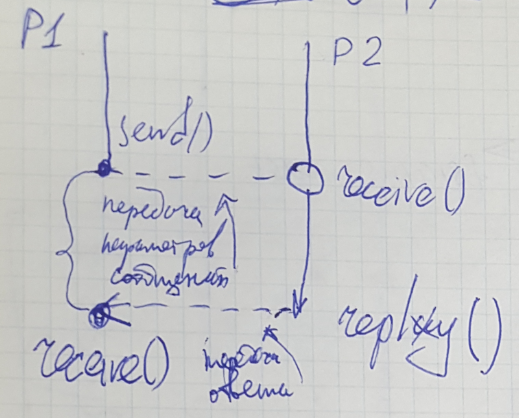
\includegraphics[width=\textwidth]{pic/1.png}
    \caption{pic}
\end{figure}

Выделяются три состояния блокировки процесса при передаче и приеме сообщений.

\begin{figure}[H]
    \centering
    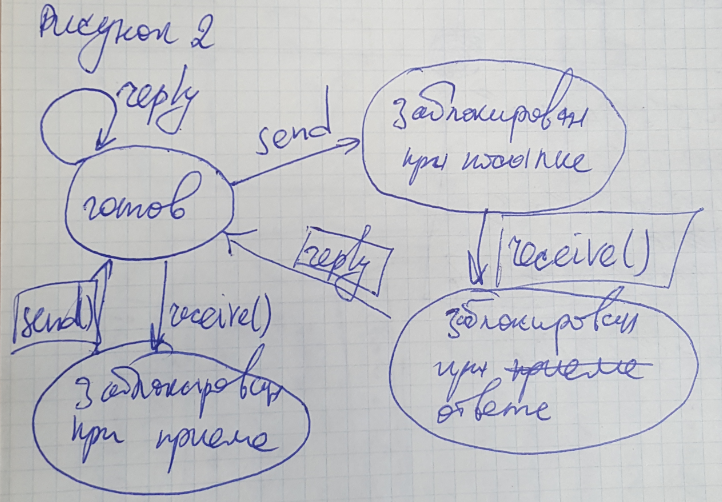
\includegraphics[width=\textwidth]{pic/2.png}
    \caption{ диаграмма три состояния блокировки при передаче сообщения}
    \label{pic:diag_3_state}
\end{figure}

На \ref{pic:diag_3_state} в рамочке – системные вызовы, выполненные другим процессом. Все три состояния блокировки могут возникнуть при строгом протоколе взаимодействия, когда процесс должен ждать.
Параметры в сигнатуре функций позволяет на этапе компиляции контролировать правильность типов.